\documentclass[border=2pt]{standalone}
\usepackage{tikz}
\usetikzlibrary{positioning}
\begin{document}
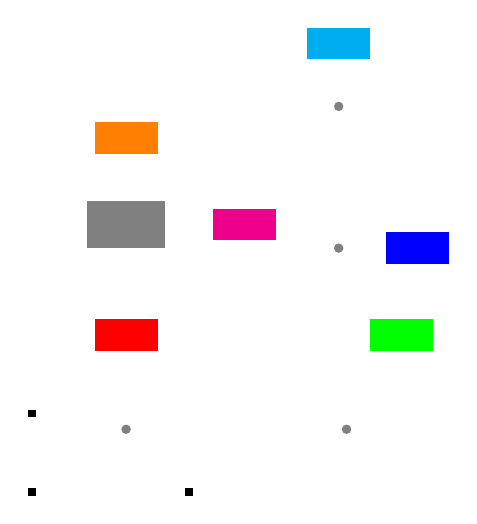
\begin{tikzpicture}[y=2cm,
  base/.style={fill=gray,minimum width=10mm,minimum height=6mm,inner sep=0pt,outer sep=0pt},
  probe/.style={minimum width=8mm,minimum height=4mm,inner sep=0pt,outer sep=0pt}]
  \fill (-.5mm,-.5mm) rectangle (.5mm,.5mm);
  \fill (19.5mm,-.5mm) rectangle (20.5mm,.5mm);
  \fill (-.5mm,9.5mm) rectangle (.5mm,10.5mm);
  \fill[gray] (12mm,8mm) circle[radius=.6mm];
  \fill[gray] (40mm,8mm) circle[radius=.6mm];
  \fill[gray] (39mm,31mm) circle[radius=.6mm];
  \fill[gray] (39mm,49mm) circle[radius=.6mm];
  \node[base] (A) at (12mm,34mm) {};
  \node[probe,fill=red,above=.5] at (12mm,8mm) {};
  \node[probe,fill=green,above right=.5 and 3mm] at (40mm,8mm) {};
  \node[probe,fill=blue,right=6mm of A] at (39mm,31mm) {};
  \node[probe,fill=magenta] at (39mm,38mm) [right=6mm of A] {};
  \node[probe,fill=orange,at={(39mm,49mm)},above=6mm of A] {};
  \node[probe,fill=cyan,above=6mm of A,at={(39mm,49mm)}] {};
\end{tikzpicture}
\end{document}
